% XXX Jedes Jahr Professoren-Texte aktualisieren!
\section[Eure Profs stellen sich vor]{Eure Professoren stellen sich vor}
\textbf{Auf den folgenden zwei Seiten stellen sich eure beiden Professoren vor.
    Sie werden gemeinsam die "Physik~1" bis "Physik~3" lesen.
    Prof.\ Thiele sowie Prof.\ Wittkowski werden sich dabei um die theoretischen und Prof.\ Fallnich um die experimentellen Aspekte des Studiums kümmern.
    Zudem stellt sich Prof.\ Wulkenhaar vor, der die Vorlesungen "Mathematik für Studierende der Physik" halten wird (ebenfalls über drei Semester).
	Da diese drei Professoren euch eine Zeit lang begleiten werden, ist es durchaus interessant zu wissen, was sie gemacht haben, bevor sie an die Uni Münster kamen, und wie ihre aktuelle Forschung aussieht.}

\begin{multicols}{2}
Liebe Erstsemesterstudentinnen und -studenten, fühlen Sie sich herzlich willkommen! Wir -- also Ihr Physik-Lehr-Team 2023 bis 2025 -- freuen uns, dass Sie eine gute Wahl getroffen und sich für ein Physikstudium an der Universität Münster entschieden haben. In den nächsten drei Semestern bieten wir Ihnen die Möglichkeit, sich regelmä{\ss}ig in den Vorlesungen Physik 1 bis 3 zu treffen, um sich durch die Themenfelder Mechanik, spezielle Relativitätstheorie, Thermodynamik sowie Elektrostatik und -dynamik bis hin zur Optik führen zu lassen. Dabei werden Prof.\ Fallnich für den experimentellen sowie Prof.\ Thiele und Prof.\ Wittkowski für den theoretischen Teil verantwortlich sein. Unsere Aufgabe ist es, Ihnen zu vermitteln, wie Sie sich die Physik und die zugehörigen inneren Zusammenhänge z.B. über Symmetriebetrachtungen systematisch erarbeiten können. Hierfür werden Ihnen die oben genannten Themenbereiche sowohl in Theorie als auch Experiment mit regelmä{\ss}igem wechselseitigem Bezug zueinander nähergebracht. Zur ersten Anwendung und auch Vertiefung Ihres erlernten Wissens wird Privatdozent Kovarik zusammen mit Übungs\-gruppen\-leiter\-innen und -leitern einen Übungsbetrieb umsetzen, durch den Sie anhand ausgewählter Beispielaufgaben die fachlichen Inhalte stärker im Detail kennenlernen werden. Für die Vorbereitung und Ausführung instruktiver Experimente in der Vorlesung ist Herr Horstmann zuständig.

Damit Sie wissen, mit welchen Dozenten Sie es direkt zu tun haben werden, möchten wir uns Ihnen gern kurz vorstellen:

Prof.\ Raphael Wittkowski ist für den theoretischen Kursteil mitverantwortlich. Er arbeitet seit 2016 an der Universität Münster und forscht auf den Gebieten der Aktiven weichen Materie und der Statistischen Physik. Aktive weiche Materie besteht aus Teilchen, die sich selbstständig fortbewegen können, wie Mikroorganismen und Mikroroboter. Die Statistische Physik befasst sich mit der Beschreibung von Vielteilchensystemen. Seine Freizeit verbringt er gern in der Natur.

Prof.\ Uwe Thiele hat in den 1990ern Physik studiert, um herauszufinden, "was die Welt im Innersten zusammenhält". Nach einer ersten Tendenz in Richtung Elementarteilchenphysik, richtete sich sein Interesse aber schnell auf die Physik strukturbildender Systeme, an denen er auch heute noch mit ungebrochen großem Interesse forscht. Nach zahlreichen Forschungs- und Lehraufenthalten an verschiedenen Standorten im In- und Ausland verlagerte er vor ca.\ 10 Jahren seine Aktivitäten an die Universität Münster, wo seine Gruppe universelle Eigenschaften komplexer Nichtgleichgewichtssysteme mit analytischen und numerischen Methoden erforscht. Aufgrund vieler nichtlinear wechselwirkender Komponenten können Selbstorganisationsprozesse entstehen, die zur spontanen Entwicklung von räumlichen und zeitlichen Strukturen führen, die also nicht von au{\ss}en aufgeprägt werden. Im alltäglichen Leben zeigen sich solche Phänomene z.B. als Konvektionszellen im Milchkaffee, bei der Ausbildung von Mustern und Strukturen in der Tier- und Pflanzenwelt, und in der Dynamik von Wasserwellen, Sanddünen oder Wolkenbändern. Von gro{\ss}em aktuellem Interesse sind Tropfen komplexer Flüssigkeiten auf festen oder weichen Substraten, die Dynamik biologischer Zellen, die Entwicklung von Bakterienkolonien und allgemein die datengetriebene Modellierung.

\end{multicols}
\begin{center}
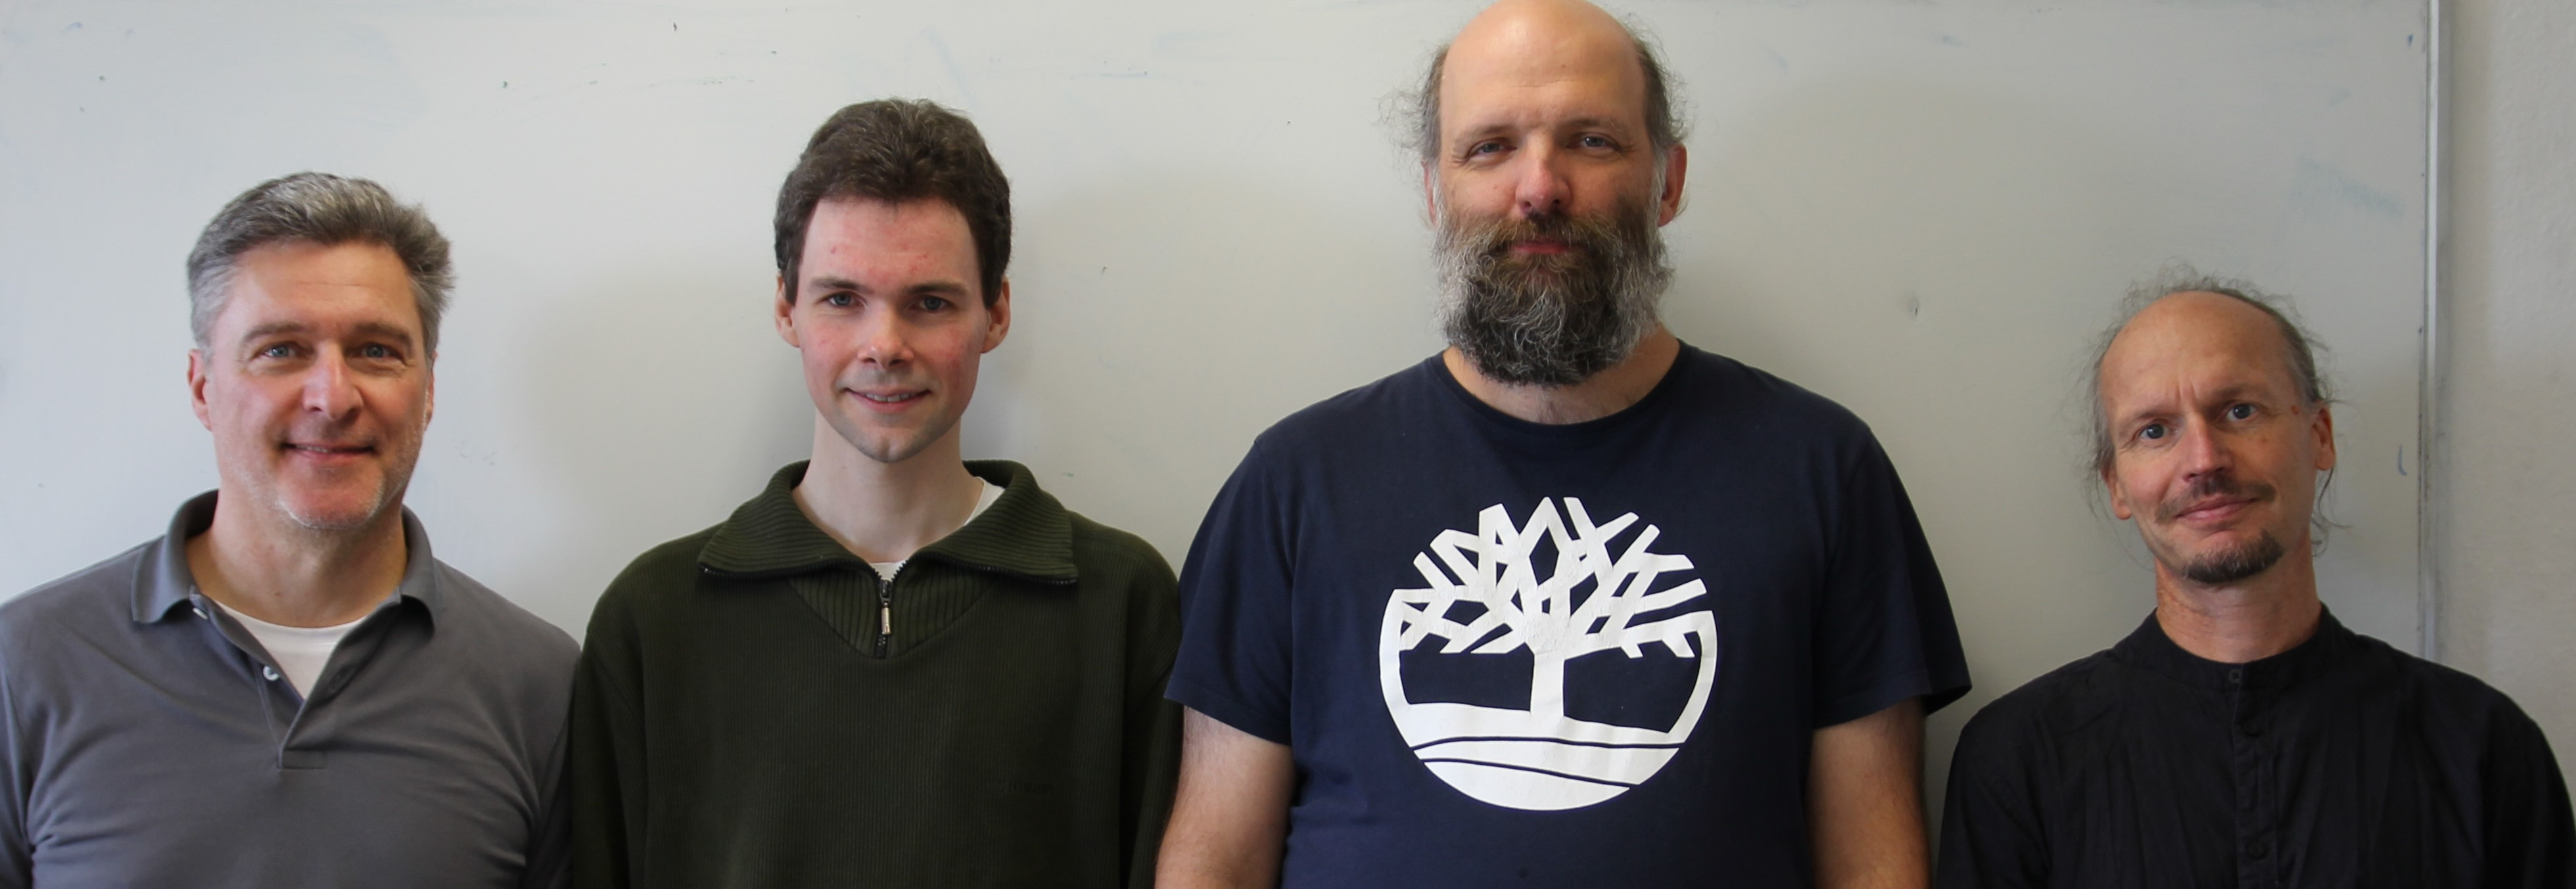
\includegraphics[width=0.6\columnwidth, height=0.25\textheight]{res/vorstellungsfotos/profs_ws23.jpg}\\
\smallskip
Gruppenfoto der Physik~1-3 Dozenten; in Ihrem Bezugssystem von links nach rechts: Carsten~Fallnich, Raphael~Wittkowski, Karol~Kovarik und Uwe~Thiele.
\end{center}

\newpage

\begin{multicols}{2}

Prof.\ Carsten Fallnich wird sich um den experimentellen Kursteil kümmern und mit Experimenten und zugehörigen Erklärungen den theoretischen Vorlesungsstoff veranschaulichen und damit weitergehend vertiefen. Er kann auf mehr als drei Jahrzehnte Wissen und Erfahrung aus Forschung und Entwicklung zurückgreifen, davon zahlreiche auch außerhalb der Universität und seit 2006 in Münster. Er ist international anerkannter Experte in der Erzeugung und Anwendung von ultrakurzen Lichtimpulsen und der nichtlinearen Optik in Wellenleitern für die zukunftsweisende Photonik, welche nahezu alle Disziplinen der modernen Physik verbindet. Neben der Arbeit an der Universität verbringt Carsten Fallnich soweit wie möglich Zeit mit der Familie, joggt, fotografiert, fährt Zweiräder mit und ohne Motor und repariert (zumindest immer mit Erkenntnisgewinn!) aus Interesse an Nachhaltigkeit und Technikverständnis fast alles, was ihm ohne reguläre Funktion unter die Finger kommt.

Priv.-Doz.~Karol Kovarik organisiert den Übungsbetrieb in den Kursen Physik 1-3. Er bietet auch verschiedene freiwillige Angebote an, um Ihnen den Einstieg in die Physik zu erleichtern und um Ihnen die Gelegenheit zu geben, zusätzliche Fragen zu den Inhalten der Vorlesungen und übungen zu stellen. Seit seiner Promotion in 2006 forscht er im Feld der Elementar- und Astroteilchenphysik. Besonders spannend findet er die Suche nach der gro{\ss}en vereinheitlichten Theorie und Versuche, die innere Struktur des Protons zu verstehen. Wenn er nachts nicht schlafen kann, fotografiert er nächtliche Landschaften und den Sternenhimmel.

Das Verständnis komplexer Phänomene, welche das Leben in unserer Welt erst interessant gestalten und an denen z.B. viele  Arbeitsgruppen am Fachbereich Physik forschen, baut -- ob Sie es uns (schon jetzt) abnehmen mögen oder nicht -- auf den Inhalten der Grundvorlesungen auf, die nun auf Sie warten. Den notwendigen Stoffumfang dazu werden Sie sich mit Interesse, Motivation und Einsatz erfolgreich selbstständig unter unserer Anleitung aneignen können; dafür wünschen wir Ihnen Durchhaltevermögen, Freude und Erfolg. Denn es wird sich später für Sie in verschiedenster Weise auszahlen, in physikalischer Weise denken und handeln zu können. Sollten dann doch noch zwischendrin Fragen offen bleiben oder Sie sich bereits für Näheres zu unseren Forschungsarbeiten interessieren, kontaktieren Sie uns gerne unter den folgenden Kontaktdaten:\\

\begin{itemize}
\item Prof.\ Dr.\ Carsten Fallnich, Institut für Angewandte Physik (AP), Büro 210, Tel.: +49\,251~83-36160, Email: \email{fallnich@uni-muenster.de} \\ \url{https://kurzelinks.de/fallnich} 

\item Prof.\ Dr.\ Uwe Thiele, Institut für Theoretische Physik (ITP), Büro 315,  Tel.: +49\,251~83-34939, Email: \email{u.thiele@uni-muenster.de} \\ \url{https://kurzelinks.de/Thiele} 

\item Priv.\ Doz.\ Dr.\ Karol Kovarik, Institut für Theoretische Physik (ITP), Büro 320, Tel.: +49\,251~83-34920, Email: \email{karol.kovarik@uni-muenster.de} \\ \url{https://kurzelinks.de/kovarik} 

\item Prof.\ Dr.\ Raphael Wittkowski, Center of Soft Nanoscience (SoN), Büro 120.024, Tel.: +49\,251~83-34529, Email: \email{raphael.wittkowski@uni-muenster.de} \\ \url{https://www.uni-muenster.de/Physik.TP/research/wittkowski} 
\end{itemize}

\begin{center}
\includegraphics[width=0.8\columnwidth]{private/res/comics/manchmal_edited.jpg}\\
{\footnotesize 
S.~Harris – \url{sciencecartoonsplus.com}
}
\end{center}

\end{multicols}

\vfill

\newpage

\begin{multicols}{2}
\begin{center}
	% 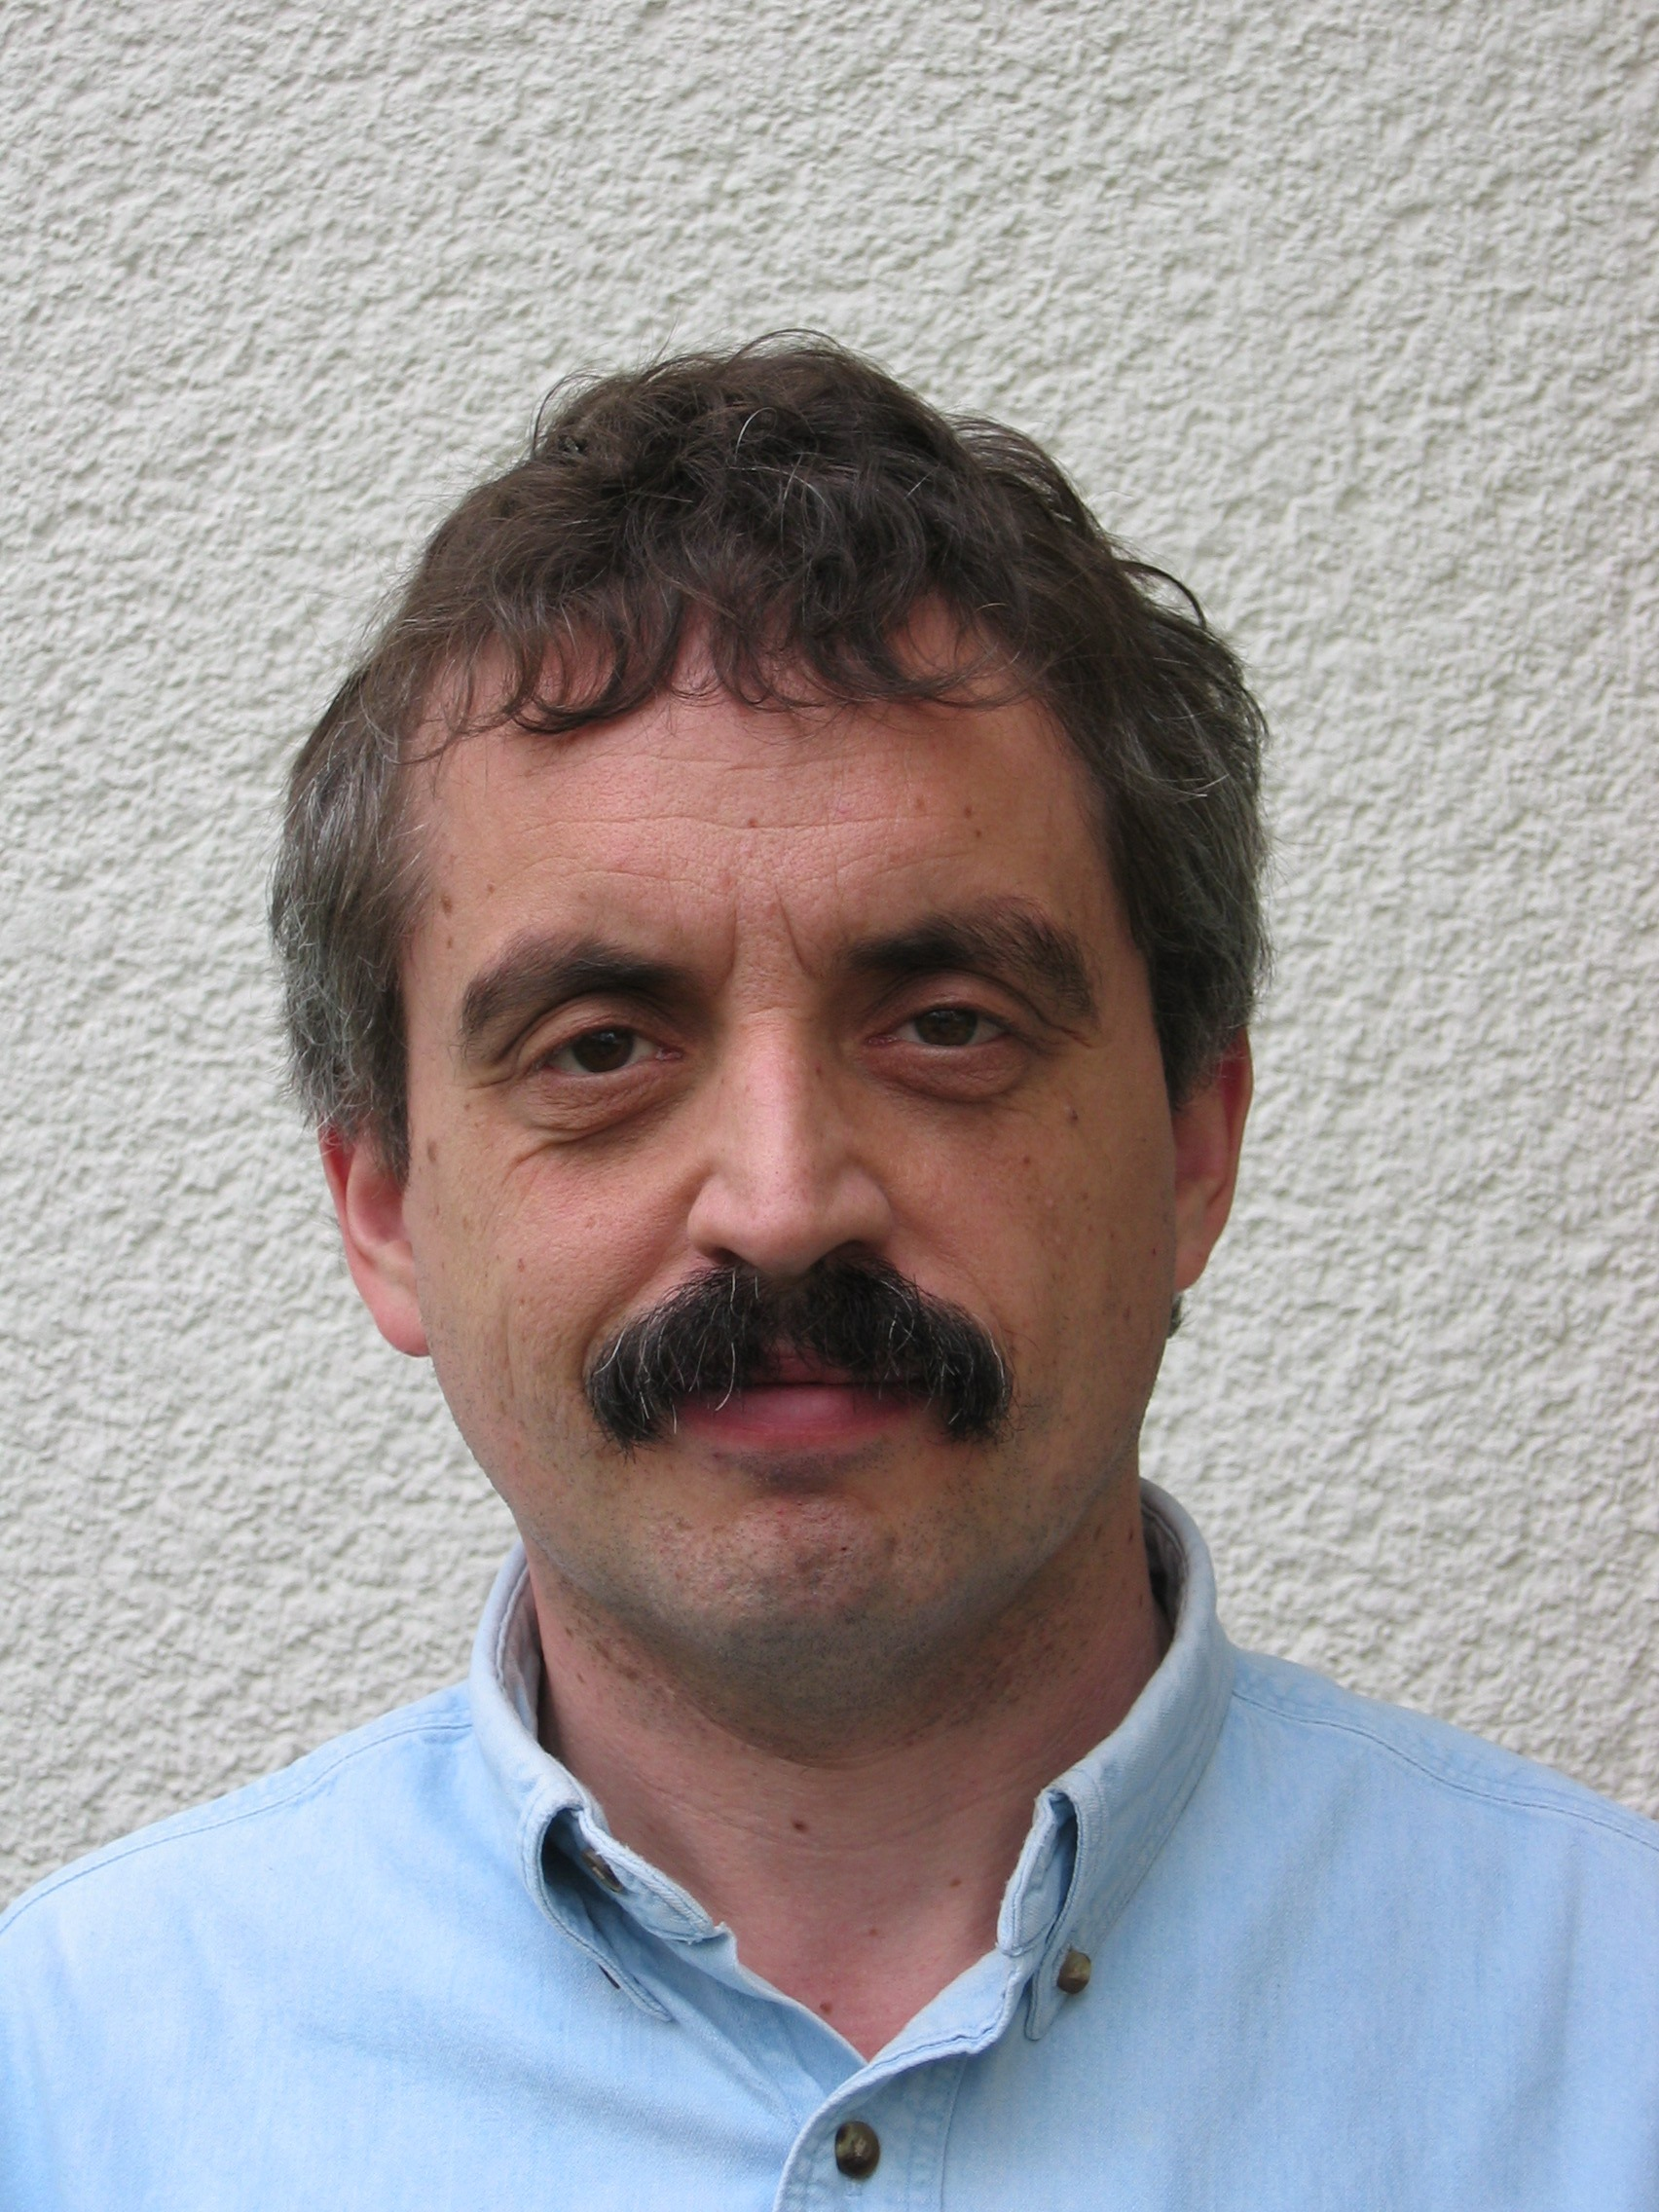
\includegraphics[width=\columnwidth, height=0.35\textheight]{res/vorstellungsfotos/wend_werner.jpg}\\
	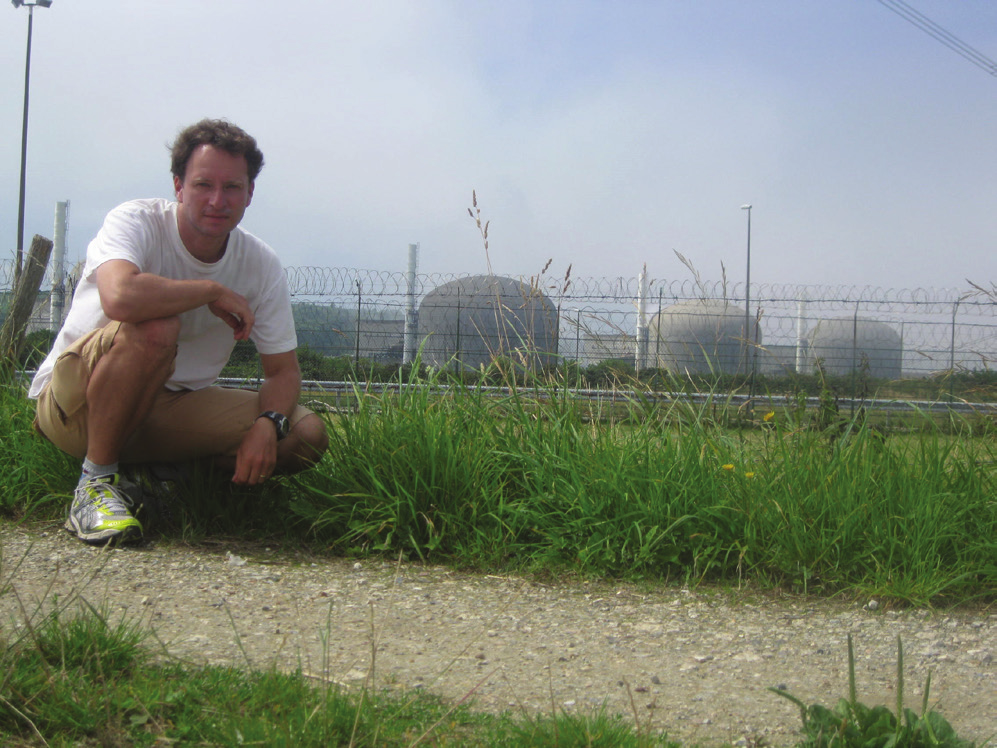
\includegraphics[width=\columnwidth, height=0.35\textheight]{res/vorstellungsfotos/wulkenhaar.png}\\
	\smallskip
 	Prof.\ Dr.\ Raimar Wulkenhaar\\
	Mathematisches Institut
\end{center}

Ich bin von der Ausbildung her Physiker, arbeite im Grenzgebiet zwischen Mathematik und Physik und bin seit 2005 Professor für Reine Mathematik am Fachbereich Mathematik und Informatik der WWU.

Die Vorlesung "Mathematik für Physiker" wird traditionell vom Mathematischen Institut veranstaltet. Es ist aus meiner Sicht eine schöne Vorlesung; mir ist aber klar, dass die meisten Studierenden das anders sehen.

Auch wenn der Stoff durchaus umfangreich ist, können wir nur einen kleinen Teil dessen behandeln, was die Physik benötigt. Es geht in der Vorlesung nicht um die Bereitstellung von Rechenwerkzeugen für die Physik; das bekommen Sie nebenbei in den Physikvorlesungen geliefert. Es geht in der Mathematik darum zu verstehen, weshalb diese Rechenwerkzeuge so und nicht anders funktionieren. Der Einstieg in die Denkweise der Mathematik ist für viele nicht leicht. Erst im Lauf der Zeit entsteht rückblickend ein gewisses Verständnis für die tiefliegenden Strukturen und Zusammenhänge der Mathematik. Im Idealfall gelangen Sie so zu einer soliden Grundlage, mit der Sie die Rechenwerkzeuge der Physik nicht nur verstehend nutzen, sondern kreativ weiterentwickeln können.


\[
\resizebox{0.45\hsize}{!}{$\displaystyle\sum_{n = 1}^\infty \frac{1}{n^2} = \frac{\pi^2}{6}$}
\]

Nun noch einige Informationen zu mir. Nach Physikstudium an der Universität Leipzig mit Abschluss als Diplomphysiker. 1994 habe ich in Leipzig auch meine Doktorarbeit geschrieben und 1997 verteidigt. Dabei ging es um die Formulierung von Modellen der Teilchenphysik im Rahmen der nichtkommutativen Geometrie. Die Ergebnisse sind rückblickend völlig unwichtig, sie haben mich aber 1998/1999 als DAAD-Postdoc nach Marseille gebracht.

Ich habe am Centre de Physique Theorique in Marseille mein Arbeitsgebiet gefunden, die Quantenfeldtheorie auf nichtkommutativen Geometrien. Vereinfacht gesagt geht es um die Frage (und ihre Konsequenzen), ob man auf beliebig kleinen Längenskalen, sagen wir $10^{-80}$\,m, noch Physik betreiben kann. Es gibt gute Gründe anzunehmen, dass das unmöglich ist, und entsprechend sollte zur Formulierung physikalischer Gesetze eine Geometrie benutzt werden, in der $10^{-80}$\,m ebenfalls sinnlos sind. Diese Nichtkommutative Geometrie wird in einer Sprache analog zur Quantenphysik beschrieben.

Seit Marseille, vor allem aber seit meiner zweiten Postdoc-Station 2000/2001 an der Universität Wien, arbeite ich an quantenfeldtheoretischen Modellen auf einer besonders einfachen nichtkommutativen Geometrie. Während meines dritten Postdoc-Aufenthalts 2002/2005 am Max- Planck-Institut für Mathematik in den Naturwissenschaften in Leipzig konnte ich mit meinem Kollegen aus Wien zusammen eine größere Hürde beseitigen. Die mathematisch rigorose Konstruktion einer 4-dimensionalen Quantenfeldtheorie auf einer nichtkommutativen Geometrie konnten wir inzwischen abschließen. Etwas analoges ist in der üblichen kommutativen Geometrie bisher nicht geglückt. Es resultierten spannende Fragen, an denen ich seitdem arbeite.

\begin{center}
	%\fibelimgtext{
		%\includegraphics[width=0.85\textwidth]{res/xkcd/435_purity.png}
	%}{\url{https://xkcd.com/435}}
 	\includegraphics[width=0.85\columnwidth]{private/res/comics/calvin_mathe.pdf}
\end{center}

\end{multicols}
